\documentclass{article}\usepackage[]{graphicx}\usepackage[]{color}
%% maxwidth is the original width if it is less than linewidth
%% otherwise use linewidth (to make sure the graphics do not exceed the margin)
\makeatletter
\def\maxwidth{ %
  \ifdim\Gin@nat@width>\linewidth
    \linewidth
  \else
    \Gin@nat@width
  \fi
}
\makeatother

\definecolor{fgcolor}{rgb}{0.345, 0.345, 0.345}
\newcommand{\hlnum}[1]{\textcolor[rgb]{0.686,0.059,0.569}{#1}}%
\newcommand{\hlstr}[1]{\textcolor[rgb]{0.192,0.494,0.8}{#1}}%
\newcommand{\hlcom}[1]{\textcolor[rgb]{0.678,0.584,0.686}{\textit{#1}}}%
\newcommand{\hlopt}[1]{\textcolor[rgb]{0,0,0}{#1}}%
\newcommand{\hlstd}[1]{\textcolor[rgb]{0.345,0.345,0.345}{#1}}%
\newcommand{\hlkwa}[1]{\textcolor[rgb]{0.161,0.373,0.58}{\textbf{#1}}}%
\newcommand{\hlkwb}[1]{\textcolor[rgb]{0.69,0.353,0.396}{#1}}%
\newcommand{\hlkwc}[1]{\textcolor[rgb]{0.333,0.667,0.333}{#1}}%
\newcommand{\hlkwd}[1]{\textcolor[rgb]{0.737,0.353,0.396}{\textbf{#1}}}%

\usepackage{framed}
\makeatletter
\newenvironment{kframe}{%
 \def\at@end@of@kframe{}%
 \ifinner\ifhmode%
  \def\at@end@of@kframe{\end{minipage}}%
  \begin{minipage}{\columnwidth}%
 \fi\fi%
 \def\FrameCommand##1{\hskip\@totalleftmargin \hskip-\fboxsep
 \colorbox{shadecolor}{##1}\hskip-\fboxsep
     % There is no \\@totalrightmargin, so:
     \hskip-\linewidth \hskip-\@totalleftmargin \hskip\columnwidth}%
 \MakeFramed {\advance\hsize-\width
   \@totalleftmargin\z@ \linewidth\hsize
   \@setminipage}}%
 {\par\unskip\endMakeFramed%
 \at@end@of@kframe}
\makeatother

\definecolor{shadecolor}{rgb}{.97, .97, .97}
\definecolor{messagecolor}{rgb}{0, 0, 0}
\definecolor{warningcolor}{rgb}{1, 0, 1}
\definecolor{errorcolor}{rgb}{1, 0, 0}
\newenvironment{knitrout}{}{} % an empty environment to be redefined in TeX

\usepackage{alltt}
\usepackage{enumerate}
\usepackage{amsmath}
\IfFileExists{upquote.sty}{\usepackage{upquote}}{}
\begin{document}

\title{\huge \textbf{Stat 207 HW6} \\}
\author{\large Cheng Luo 912466499 \\ \large Fan Wu 912538518}
\maketitle

\newpage
\mbox{}
\newpage

\section{14.9}

\begin{enumerate}[(a)]

\item

\begin{knitrout}
\definecolor{shadecolor}{rgb}{0.969, 0.969, 0.969}\color{fgcolor}\begin{kframe}
\begin{alltt}
  \hlstd{dat} \hlkwb{=} \hlkwd{read.table}\hlstd{(}\hlstr{"CH14PR09.txt"}\hlstd{)}
  \hlkwd{names}\hlstd{(dat)} \hlkwb{=} \hlkwd{c}\hlstd{(}\hlstr{"Y"}\hlstd{,} \hlstr{"X"}\hlstd{)}
  \hlstd{logit} \hlkwb{=} \hlkwd{glm}\hlstd{(Y} \hlopt{~} \hlstd{X,} \hlkwc{data} \hlstd{= dat,} \hlkwc{family} \hlstd{=} \hlstr{"binomial"}\hlstd{)}
  \hlkwd{summary}\hlstd{(logit)}
\end{alltt}
\begin{verbatim}
## 
## Call:
## glm(formula = Y ~ X, family = "binomial", data = dat)
## 
## Deviance Residuals: 
##     Min       1Q   Median       3Q      Max  
## -1.7845  -0.8350   0.5065   0.8371   1.7145  
## 
## Coefficients:
##               Estimate Std. Error z value Pr(>|z|)  
## (Intercept) -10.308925   4.376997  -2.355   0.0185 *
## X             0.018920   0.007877   2.402   0.0163 *
## ---
## Signif. codes:  0 '***' 0.001 '**' 0.01 '*' 0.05 '.' 0.1 ' ' 1
## 
## (Dispersion parameter for binomial family taken to be 1)
## 
##     Null deviance: 37.393  on 26  degrees of freedom
## Residual deviance: 29.242  on 25  degrees of freedom
## AIC: 33.242
## 
## Number of Fisher Scoring iterations: 4
\end{verbatim}
\end{kframe}
\end{knitrout}

\qquad From the summary, the maximum likelihood estimates of $\hat{\beta}_0 = -10.308925$, $\hat{\beta}_1 = 0.018920$, $$\hat{\pi} = \frac{exp(\beta_0+\beta_1 X)}{1+exp(\beta_0+\beta_1 X)}=\frac{exp(-10.308925+0.018920 X)}{1+exp(-10.308925+0.018920 X)}$$

\item

\begin{knitrout}
\definecolor{shadecolor}{rgb}{0.969, 0.969, 0.969}\color{fgcolor}\begin{kframe}
\begin{alltt}
  \hlkwd{plot}\hlstd{(dat}\hlopt{$}\hlstd{X,} \hlkwd{fitted}\hlstd{(logit),} \hlkwc{ylim} \hlstd{=} \hlkwd{c}\hlstd{(}\hlnum{0}\hlstd{,} \hlnum{1}\hlstd{))}
  \hlkwd{points}\hlstd{(dat}\hlopt{$}\hlstd{X, dat}\hlopt{$}\hlstd{Y,} \hlkwc{lwd} \hlstd{=} \hlnum{9}\hlstd{)}
  \hlkwd{lines}\hlstd{(}\hlkwd{lowess}\hlstd{(dat}\hlopt{$}\hlstd{Y} \hlopt{~} \hlstd{dat}\hlopt{$}\hlstd{X),} \hlkwc{lty} \hlstd{=} \hlnum{2}\hlstd{)}
\end{alltt}
\end{kframe}
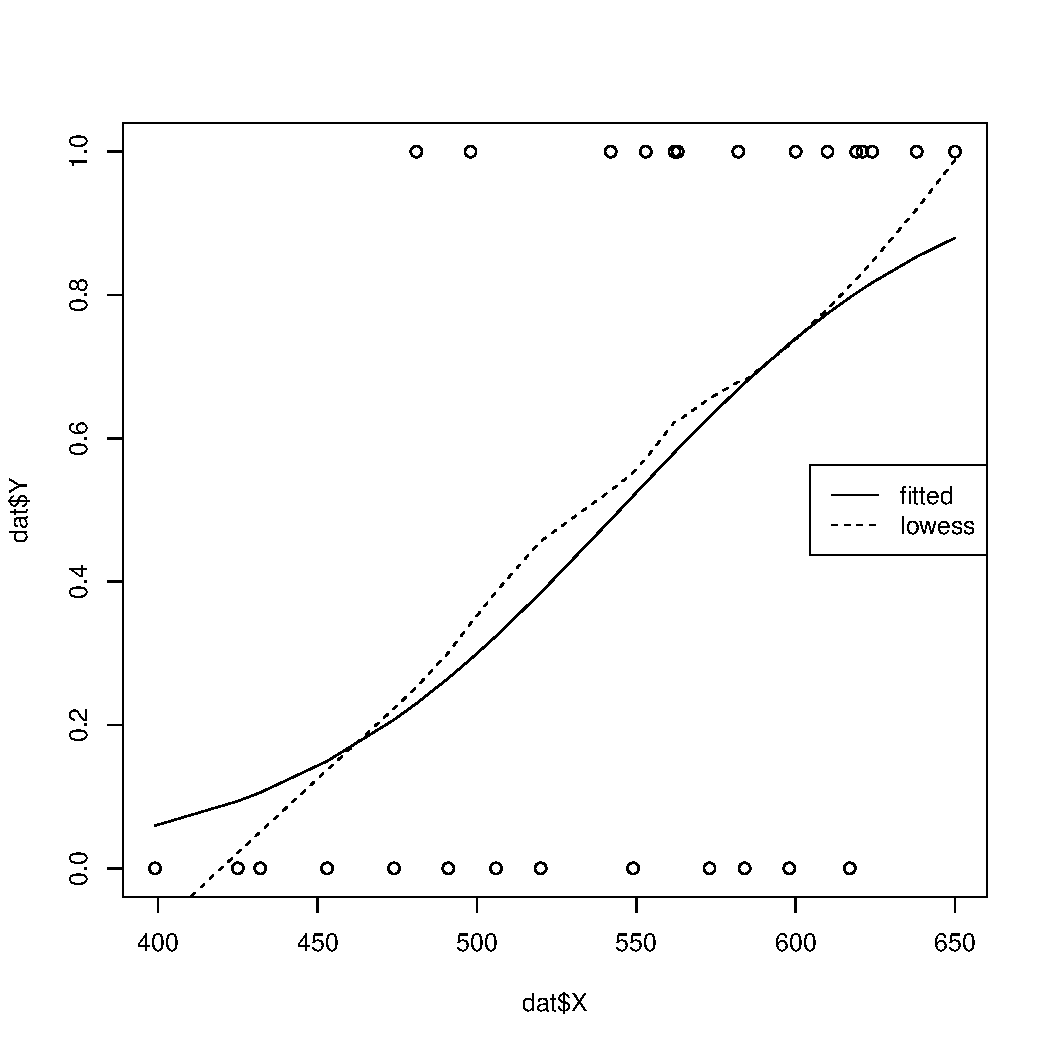
\includegraphics[width=\maxwidth]{figure/unnamed-chunk-2-1} 

\end{knitrout}

\qquad The fitted logistic response function appears to be well.

\item

\begin{knitrout}
\definecolor{shadecolor}{rgb}{0.969, 0.969, 0.969}\color{fgcolor}\begin{kframe}
\begin{alltt}
  \hlkwd{exp}\hlstd{(}\hlnum{0.018920}\hlstd{)}
\end{alltt}
\begin{verbatim}
## [1] 1.0191
\end{verbatim}
\end{kframe}
\end{knitrout}

\qquad $exp(\beta_1)=1.0191$, so that the odds of employee's ability increased by 1.91\% with each additional employee's emotional stability.

\item

\begin{knitrout}
\definecolor{shadecolor}{rgb}{0.969, 0.969, 0.969}\color{fgcolor}\begin{kframe}
\begin{alltt}
  \hlstd{newdat} \hlkwb{=} \hlkwd{data.frame}\hlstd{(}\hlkwc{X} \hlstd{=} \hlnum{550}\hlstd{)}
  \hlkwd{predict}\hlstd{(logit,} \hlkwc{newdata} \hlstd{= newdat,} \hlkwc{type} \hlstd{=} \hlstr{"response"}\hlstd{)}
\end{alltt}
\begin{verbatim}
##         1 
## 0.5242263
\end{verbatim}
\end{kframe}
\end{knitrout}

\qquad The estimated probability that employees with an emotional stability test score of 550 will be able to perform in a task group is 0.5242263 .

\item

\begin{knitrout}
\definecolor{shadecolor}{rgb}{0.969, 0.969, 0.969}\color{fgcolor}\begin{kframe}
\begin{alltt}
  \hlstd{newpi} \hlkwb{=} \hlnum{0.7}
  \hlstd{pi_2} \hlkwb{=} \hlkwd{log}\hlstd{(newpi}\hlopt{/}\hlstd{(}\hlnum{1}\hlopt{-}\hlstd{newpi))}
  \hlstd{(pi_2} \hlopt{-} \hlstd{(}\hlopt{-}\hlnum{10.308925}\hlstd{))}\hlopt{/}\hlnum{0.018920}
\end{alltt}
\begin{verbatim}
## [1] 589.6524
\end{verbatim}
\end{kframe}
\end{knitrout}

\qquad The emotional stability test score for which 70 percents of the employees with this test score are expected to be able to  perform in a task group is 598.6524.

\end{enumerate}

\section{14.11}

\begin{enumerate}[(a)]

\item

\begin{knitrout}
\definecolor{shadecolor}{rgb}{0.969, 0.969, 0.969}\color{fgcolor}\begin{kframe}
\begin{alltt}
  \hlstd{dat} \hlkwb{=} \hlkwd{read.table}\hlstd{(}\hlstr{"CH14PR11.txt"}\hlstd{)}
  \hlkwd{names}\hlstd{(dat)} \hlkwb{=} \hlkwd{c}\hlstd{(}\hlstr{"X"}\hlstd{,} \hlstr{"n"}\hlstd{,} \hlstr{"Y"}\hlstd{)}
  \hlkwd{plot}\hlstd{(dat}\hlopt{$}\hlstd{X, dat}\hlopt{$}\hlstd{Y}\hlopt{/}\hlstd{dat}\hlopt{$}\hlstd{n)}
\end{alltt}
\end{kframe}
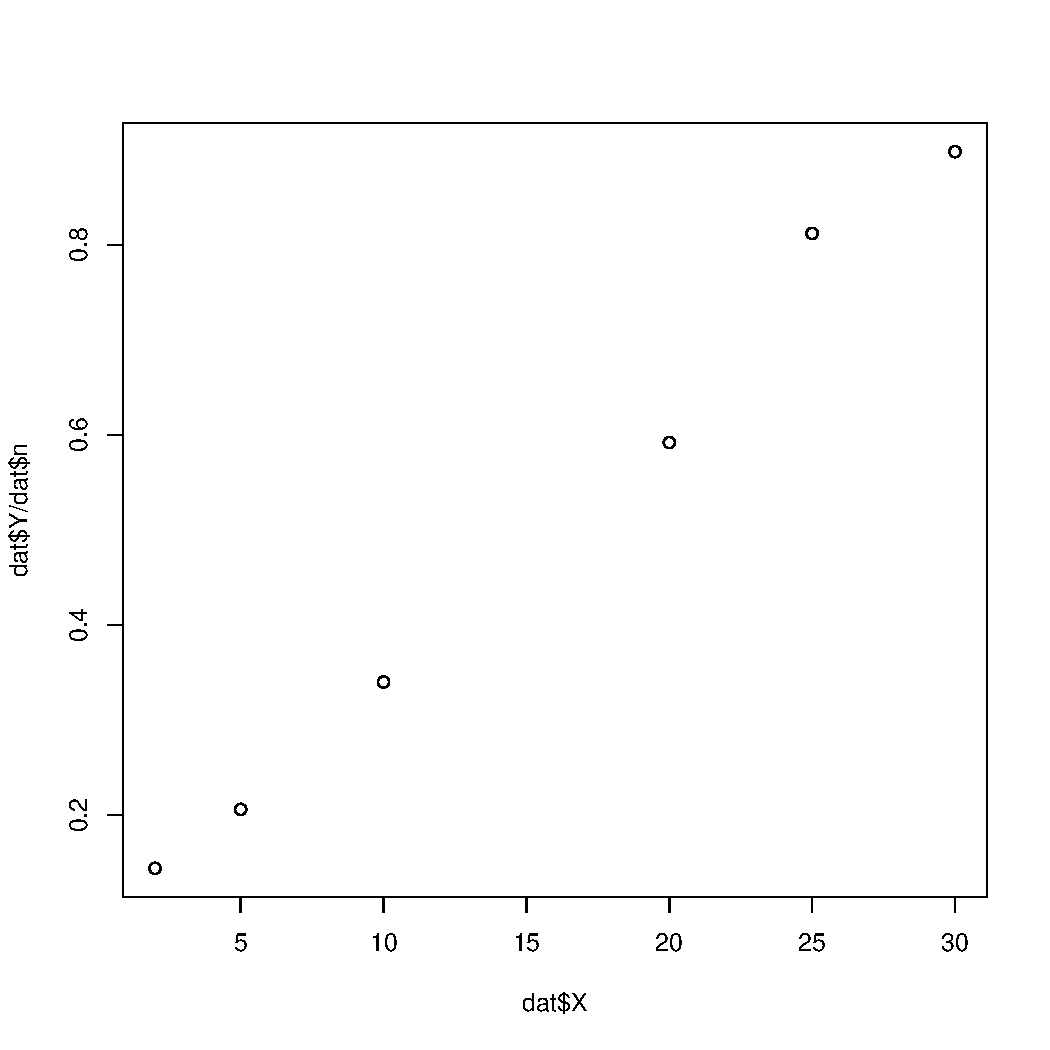
\includegraphics[width=\maxwidth]{figure/unnamed-chunk-6-1} 

\end{knitrout}

\qquad The plot support the analyst's belief that the logistic response functiion is appropriate.

\item

\begin{knitrout}
\definecolor{shadecolor}{rgb}{0.969, 0.969, 0.969}\color{fgcolor}\begin{kframe}
\begin{alltt}
  \hlstd{logit} \hlkwb{=} \hlkwd{glm}\hlstd{(Y}\hlopt{/}\hlstd{n} \hlopt{~} \hlstd{X,} \hlkwc{data} \hlstd{= dat,} \hlkwc{family} \hlstd{=} \hlstr{"binomial"}\hlstd{)}
\end{alltt}


{\ttfamily\noindent\color{warningcolor}{\#\# Warning: non-integer \#successes in a binomial glm!}}\begin{alltt}
  \hlkwd{summary}\hlstd{(logit)}
\end{alltt}
\begin{verbatim}
## 
## Call:
## glm(formula = Y/n ~ X, family = "binomial", data = dat)
## 
## Deviance Residuals: 
##         1          2          3          4          5          6  
##  0.007846   0.019363   0.025865  -0.130556   0.056842   0.054601  
## 
## Coefficients:
##             Estimate Std. Error z value Pr(>|z|)
## (Intercept)  -2.0766     1.8970  -1.095    0.274
## X             0.1359     0.1067   1.273    0.203
## 
## (Dispersion parameter for binomial family taken to be 1)
## 
##     Null deviance: 2.216343  on 5  degrees of freedom
## Residual deviance: 0.024363  on 4  degrees of freedom
## AIC: 7.1154
## 
## Number of Fisher Scoring iterations: 4
\end{verbatim}
\end{kframe}
\end{knitrout}

\qquad From the summary, the maximum likelihood estimates of $\hat{\beta}_0 = -2.0766$, $\hat{\beta}_1 = 0.1359$, $$\hat{\pi} = \frac{exp(\beta_0+\beta_1 X)}{1+exp(\beta_0+\beta_1 X)}=\frac{exp(-2.0766+0.1359 X)}{1+exp(-2.0766+0.1359 X)}$$

\item

\begin{knitrout}
\definecolor{shadecolor}{rgb}{0.969, 0.969, 0.969}\color{fgcolor}\begin{kframe}
\begin{alltt}
  \hlkwd{plot}\hlstd{(dat}\hlopt{$}\hlstd{X,} \hlkwd{fitted}\hlstd{(logit),} \hlkwc{ylim} \hlstd{=} \hlkwd{c}\hlstd{(}\hlnum{0}\hlstd{,} \hlnum{1}\hlstd{))}
  \hlkwd{points}\hlstd{(dat}\hlopt{$}\hlstd{X, dat}\hlopt{$}\hlstd{Y}\hlopt{/}\hlstd{dat}\hlopt{$}\hlstd{n,} \hlkwc{lwd} \hlstd{=} \hlnum{1}\hlstd{)}
\end{alltt}
\end{kframe}
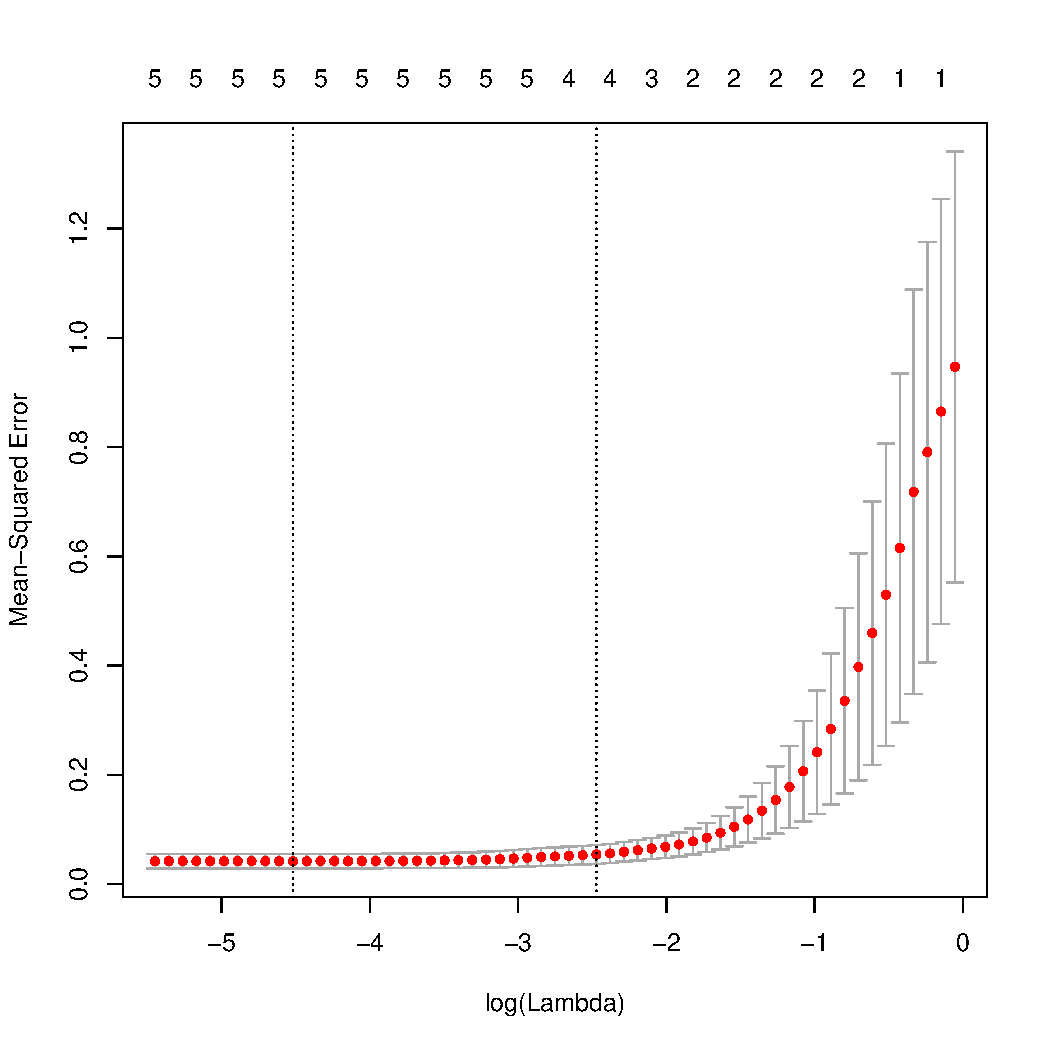
\includegraphics[width=\maxwidth]{figure/unnamed-chunk-8-1} 

\end{knitrout}

\qquad The fitted logistic response function appears to be well.

\item

\begin{knitrout}
\definecolor{shadecolor}{rgb}{0.969, 0.969, 0.969}\color{fgcolor}\begin{kframe}
\begin{alltt}
  \hlkwd{exp}\hlstd{(}\hlnum{0.1359}\hlstd{)}
\end{alltt}
\begin{verbatim}
## [1] 1.145567
\end{verbatim}
\end{kframe}
\end{knitrout}

\qquad $exp(\beta_1)=1.145567$, so that the odds of the bottles being returned is increased by 14.5567\% with each one deposit level increased.

\item

\begin{knitrout}
\definecolor{shadecolor}{rgb}{0.969, 0.969, 0.969}\color{fgcolor}\begin{kframe}
\begin{alltt}
  \hlstd{newdat} \hlkwb{=} \hlkwd{data.frame}\hlstd{(}\hlkwc{X} \hlstd{=} \hlnum{15}\hlstd{)}
  \hlkwd{predict}\hlstd{(logit,} \hlkwc{newdata} \hlstd{= newdat,} \hlkwc{type} \hlstd{=} \hlstr{"response"}\hlstd{)}
\end{alltt}
\begin{verbatim}
##         1 
## 0.4903005
\end{verbatim}
\end{kframe}
\end{knitrout}

\qquad The estimated probability that a bottle will be returned when the deposit is 15 cents is 0.4903005.

\item

\begin{knitrout}
\definecolor{shadecolor}{rgb}{0.969, 0.969, 0.969}\color{fgcolor}\begin{kframe}
\begin{alltt}
  \hlstd{newpi} \hlkwb{=} \hlnum{0.75}
  \hlstd{pi_2} \hlkwb{=} \hlkwd{log}\hlstd{(newpi}\hlopt{/}\hlstd{(}\hlnum{1}\hlopt{-}\hlstd{newpi))}
  \hlstd{(pi_2} \hlopt{-} \hlstd{(}\hlopt{-}\hlnum{2.0766}\hlstd{))}\hlopt{/}\hlnum{0.1359}
\end{alltt}
\begin{verbatim}
## [1] 23.36433
\end{verbatim}
\end{kframe}
\end{knitrout}

\qquad Estimate the amount of deposit for which 75\% of the bottles are expected to be returned is 23.36433.

\end{enumerate}

\section{14.14}

\begin{enumerate}[(a)]

\item

\begin{knitrout}
\definecolor{shadecolor}{rgb}{0.969, 0.969, 0.969}\color{fgcolor}\begin{kframe}
\begin{alltt}
  \hlstd{dat} \hlkwb{=} \hlkwd{read.table}\hlstd{(}\hlstr{"CH14PR14.txt"}\hlstd{)}
  \hlkwd{names}\hlstd{(dat)} \hlkwb{=} \hlkwd{c}\hlstd{(}\hlstr{"Y"}\hlstd{,} \hlstr{"X1"}\hlstd{,} \hlstr{"X2"}\hlstd{,} \hlstr{"X3"}\hlstd{)}
  \hlstd{logit} \hlkwb{=} \hlkwd{glm}\hlstd{(Y} \hlopt{~} \hlstd{X1} \hlopt{+} \hlstd{X2} \hlopt{+} \hlstd{X3,} \hlkwc{data} \hlstd{= dat,} \hlkwc{family} \hlstd{=} \hlstr{"binomial"}\hlstd{)}
  \hlkwd{summary}\hlstd{(logit)}
\end{alltt}
\begin{verbatim}
## 
## Call:
## glm(formula = Y ~ X1 + X2 + X3, family = "binomial", data = dat)
## 
## Deviance Residuals: 
##     Min       1Q   Median       3Q      Max  
## -1.4037  -0.5637  -0.3352  -0.1542   2.9394  
## 
## Coefficients:
##             Estimate Std. Error z value Pr(>|z|)   
## (Intercept) -1.17716    2.98242  -0.395  0.69307   
## X1           0.07279    0.03038   2.396  0.01658 * 
## X2          -0.09899    0.03348  -2.957  0.00311 **
## X3           0.43397    0.52179   0.832  0.40558   
## ---
## Signif. codes:  0 '***' 0.001 '**' 0.01 '*' 0.05 '.' 0.1 ' ' 1
## 
## (Dispersion parameter for binomial family taken to be 1)
## 
##     Null deviance: 134.94  on 158  degrees of freedom
## Residual deviance: 105.09  on 155  degrees of freedom
## AIC: 113.09
## 
## Number of Fisher Scoring iterations: 6
\end{verbatim}
\end{kframe}
\end{knitrout}

\qquad From the summary, the maximum likelihood estimates $\hat{\beta}_0 = -1.17716 $, $\hat{\beta}_1 = 0.07279$, $\hat{\beta}_2 = -0.09899 $, $\hat{\beta}_4 = 0.43397 $ $$\hat{\pi} = \frac{exp(\beta_0+\beta_1 X1 + \beta_2 X2 + \beta_3 X3)}{1+exp(\beta_0+\beta_1 X1 + \beta_2 X2 + \beta_3 X3)}=\frac{exp(-1.17716+0.07279 X1 - 0.09899 X2 +0.43397 X3)}{1+exp(-1.17716+0.07279 X1 - 0.09899 X2 +0.43397 X3)}$$

\item

\begin{knitrout}
\definecolor{shadecolor}{rgb}{0.969, 0.969, 0.969}\color{fgcolor}\begin{kframe}
\begin{alltt}
  \hlkwd{exp}\hlstd{(}\hlnum{0.07279}\hlstd{)}
\end{alltt}
\begin{verbatim}
## [1] 1.075505
\end{verbatim}
\begin{alltt}
  \hlkwd{exp}\hlstd{(}\hlopt{-}\hlnum{0.09899} \hlstd{)}
\end{alltt}
\begin{verbatim}
## [1] 0.9057518
\end{verbatim}
\begin{alltt}
  \hlkwd{exp}\hlstd{(}\hlnum{0.43397}\hlstd{)}
\end{alltt}
\begin{verbatim}
## [1] 1.543373
\end{verbatim}
\end{kframe}
\end{knitrout}

\begin{itemize}
\item
$exp(\beta_1)=1.075505$, so that the odds of getting a flu shot is increased by 7.5\% with each one age increased.
\item
$exp(\beta_2)=0.9057518$, so that the odds of getting a flu shot is decreased by 9.4\% with each one health awareness index increased.
\item
$exp(\beta_3)=1.543373$, so that the odds of getting a flu shot is increased by 54.3\% from woman to man.
\end{itemize}

\item

\begin{knitrout}
\definecolor{shadecolor}{rgb}{0.969, 0.969, 0.969}\color{fgcolor}\begin{kframe}
\begin{alltt}
  \hlstd{newdat} \hlkwb{=} \hlkwd{data.frame}\hlstd{(}\hlkwc{X1} \hlstd{=} \hlnum{55}\hlstd{,} \hlkwc{X2} \hlstd{=} \hlnum{60}\hlstd{,} \hlkwc{X3} \hlstd{=} \hlnum{1}\hlstd{)}
  \hlkwd{predict}\hlstd{(logit,} \hlkwc{newdata} \hlstd{= newdat,} \hlkwc{type} \hlstd{=} \hlstr{"response"}\hlstd{)}
\end{alltt}
\begin{verbatim}
##          1 
## 0.06422197
\end{verbatim}
\end{kframe}
\end{knitrout}

\qquad The estimated probability with X1=55, X2=60 and X3=1 is 0.06422197 .

\end{enumerate}

\section{14.19}

\begin{enumerate}[(a)]

\item

\begin{knitrout}
\definecolor{shadecolor}{rgb}{0.969, 0.969, 0.969}\color{fgcolor}\begin{kframe}
\begin{alltt}
  \hlstd{dat} \hlkwb{=} \hlkwd{read.table}\hlstd{(}\hlstr{"CH14PR13.txt"}\hlstd{)}
  \hlkwd{names}\hlstd{(dat)} \hlkwb{=} \hlkwd{c}\hlstd{(}\hlstr{"Y"}\hlstd{,} \hlstr{"X1"}\hlstd{,} \hlstr{"X2"}\hlstd{)}
  \hlstd{logit} \hlkwb{=} \hlkwd{glm}\hlstd{(Y} \hlopt{~} \hlstd{X1} \hlopt{+} \hlstd{X2,} \hlkwc{data} \hlstd{= dat,} \hlkwc{family} \hlstd{=} \hlstr{"binomial"}\hlstd{)}
  \hlkwd{summary}\hlstd{(logit)}
\end{alltt}
\begin{verbatim}
## 
## Call:
## glm(formula = Y ~ X1 + X2, family = "binomial", data = dat)
## 
## Deviance Residuals: 
##     Min       1Q   Median       3Q      Max  
## -1.6189  -0.8949  -0.5880   0.9653   2.0846  
## 
## Coefficients:
##             Estimate Std. Error z value Pr(>|z|)  
## (Intercept) -4.73931    2.10195  -2.255   0.0242 *
## X1           0.06773    0.02806   2.414   0.0158 *
## X2           0.59863    0.39007   1.535   0.1249  
## ---
## Signif. codes:  0 '***' 0.001 '**' 0.01 '*' 0.05 '.' 0.1 ' ' 1
## 
## (Dispersion parameter for binomial family taken to be 1)
## 
##     Null deviance: 44.987  on 32  degrees of freedom
## Residual deviance: 36.690  on 30  degrees of freedom
## AIC: 42.69
## 
## Number of Fisher Scoring iterations: 4
\end{verbatim}
\end{kframe}
\end{knitrout}

\item

\begin{knitrout}
\definecolor{shadecolor}{rgb}{0.969, 0.969, 0.969}\color{fgcolor}\begin{kframe}
\begin{alltt}
  \hlkwd{qnorm}\hlstd{(}\hlnum{1}\hlopt{-}\hlnum{0.05}\hlopt{/}\hlnum{2}\hlstd{)}
\end{alltt}
\begin{verbatim}
## [1] 1.959964
\end{verbatim}
\end{kframe}
\end{knitrout}

\begin{center}
$H_0$:$\beta_2=0$

VS. $H_1$:$\beta_2 \ne 0$

$z^*=\frac{b2}{s(b_2)} = 0.59863/0.39007   = 1.535$

we can reject $H_0$ if $|z^*| > Z(1-0.05/2)=1.959964$,otherwise reject$H_1$

so that reject $H_1$ because $|z^*|<1.959964$,

therefore, X2 can be dropped from the regression model, and the P-value is 0.1249 
\end{center}

\item

\begin{knitrout}
\definecolor{shadecolor}{rgb}{0.969, 0.969, 0.969}\color{fgcolor}\begin{kframe}
\begin{alltt}
  \hlkwd{logLik}\hlstd{(logit)}
\end{alltt}
\begin{verbatim}
## 'log Lik.' -18.34482 (df=3)
\end{verbatim}
\begin{alltt}
  \hlstd{logitR} \hlkwb{=} \hlkwd{glm}\hlstd{(Y} \hlopt{~} \hlstd{X1,} \hlkwc{data} \hlstd{= dat,} \hlkwc{family} \hlstd{=} \hlstr{"binomial"}\hlstd{)}
  \hlkwd{logLik}\hlstd{(logitR)}
\end{alltt}
\begin{verbatim}
## 'log Lik.' -19.65227 (df=2)
\end{verbatim}
\begin{alltt}
  \hlkwd{qchisq}\hlstd{(}\hlnum{1}\hlopt{-}\hlnum{0.05}\hlstd{,} \hlnum{3}\hlopt{-}\hlnum{2}\hlstd{)}
\end{alltt}
\begin{verbatim}
## [1] 3.841459
\end{verbatim}
\begin{alltt}
  \hlkwd{pchisq}\hlstd{(}\hlnum{2.614}\hlstd{,} \hlnum{1}\hlstd{,} \hlkwc{lower.tail} \hlstd{=} \hlnum{FALSE}\hlstd{)}
\end{alltt}
\begin{verbatim}
## [1] 0.1059243
\end{verbatim}
\end{kframe}
\end{knitrout}

\begin{center}
$H_0$:$\beta_2=0$

VS. $H_1$:$\beta_2 \ne 0$

The full model: $\pi = [1 + exp(-(\beta_0 + \beta_1 X1 + \beta_2 X2))]^{-1} $

L(F)= -18.34482

The reduced model: $\pi = [1 + exp(-(\beta_0 + \beta_1 X1))]^{-1} $

L(R)= -19.65227

$G^2$ = -2(ln(L(R)-ln(L(F)))) = 2.614

we can reject $H_0$ if $G^2 > \chi^2(1-0.05, 3-2)=3.8415$,otherwise reject$H_1$

so that reject $H_1$ because $G^2 <3.8415$,

therefore, X2 can be dropped from the regression model, and the P-value is 0.1059.And the result is same as the result we get in (b).
\end{center}

\item

\begin{knitrout}
\definecolor{shadecolor}{rgb}{0.969, 0.969, 0.969}\color{fgcolor}\begin{kframe}
\begin{alltt}
  \hlkwd{logLik}\hlstd{(logit)}
\end{alltt}
\begin{verbatim}
## 'log Lik.' -18.34482 (df=3)
\end{verbatim}
\begin{alltt}
  \hlstd{logitF} \hlkwb{=} \hlkwd{glm}\hlstd{(Y} \hlopt{~} \hlstd{X1} \hlopt{+} \hlstd{X2} \hlopt{+}\hlkwd{I}\hlstd{(X1}\hlopt{^}\hlnum{2}\hlstd{)} \hlopt{+} \hlkwd{I}\hlstd{(X2}\hlopt{^}\hlnum{2}\hlstd{)} \hlopt{+} \hlkwd{I}\hlstd{(X1}\hlopt{*}\hlstd{X2),} \hlkwc{data} \hlstd{= dat,} \hlkwc{family} \hlstd{=} \hlstr{"binomial"}\hlstd{)}
  \hlkwd{logLik}\hlstd{(logitF)}
\end{alltt}
\begin{verbatim}
## 'log Lik.' -17.12634 (df=6)
\end{verbatim}
\begin{alltt}
  \hlkwd{qchisq}\hlstd{(}\hlnum{1}\hlopt{-}\hlnum{0.05}\hlstd{,} \hlnum{6}\hlopt{-}\hlnum{3}\hlstd{)}
\end{alltt}
\begin{verbatim}
## [1] 7.814728
\end{verbatim}
\begin{alltt}
  \hlkwd{pchisq}\hlstd{(}\hlnum{2.436953}\hlstd{,} \hlnum{3}\hlstd{,} \hlkwc{lower.tail} \hlstd{=} \hlnum{FALSE}\hlstd{)}
\end{alltt}
\begin{verbatim}
## [1] 0.4867929
\end{verbatim}
\end{kframe}
\end{knitrout}

\begin{center}
$H_0$:$\beta_3=\beta_4=\beta_5=0$

VS. $H_1$:not all $\beta_k=0$,k=3,4,5

The full model: $\pi = [1 + exp(-(\beta_0 + \beta_1 X1 + \beta_2 X2 + \beta_3 X3 + \beta_4 X4 + \beta_5 X5))]^{-1} $

L(F)= -17.12634

The reduced model: $\pi = [1 + exp(-(\beta_0 + \beta_1 X1 + \beta_2 X2))]^{-1} $

L(R)= -18.34482

$G^2$ = -2(ln(L(R)-ln(L(F)))) = 2.436953

we can reject $H_0$ if $G^2 > \chi^2(1-0.05, 6-3)=7.81$,otherwise reject$H_1$

so that reject $H_1$ because $G^2 <7.81$,

therefore, X3,X4,X5 can be dropped from the regression model, and the P-value is 0.4867929.
\end{center}

\end{enumerate}

\section{Problem 5}

\begin{enumerate}[(a)]

\item

\begin{knitrout}
\definecolor{shadecolor}{rgb}{0.969, 0.969, 0.969}\color{fgcolor}\begin{kframe}
\begin{alltt}
  \hlstd{dat} \hlkwb{=} \hlkwd{read.table}\hlstd{(}\hlstr{"apartment.txt"}\hlstd{,} \hlkwc{header} \hlstd{=} \hlnum{TRUE}\hlstd{)}
  \hlkwd{require}\hlstd{(}\hlstr{"pls"}\hlstd{)}
\end{alltt}


{\ttfamily\noindent\itshape\color{messagecolor}{\#\# Loading required package: pls}}

{\ttfamily\noindent\color{warningcolor}{\#\# Warning: package 'pls' was built under R version 3.1.2}}

{\ttfamily\noindent\itshape\color{messagecolor}{\#\# \\\#\# Attaching package: 'pls'\\\#\# \\\#\# The following object is masked from 'package:stats':\\\#\# \\\#\#\ \ \ \  loadings}}\begin{alltt}
  \hlstd{dat.stan} \hlkwb{=} \hlstd{dat}
  \hlkwa{for}\hlstd{(j} \hlkwa{in} \hlnum{1}\hlopt{:}\hlkwd{ncol}\hlstd{(dat))}
    \hlstd{dat.stan[,j]} \hlkwb{=} \hlstd{(dat[,j]} \hlopt{-} \hlkwd{mean}\hlstd{(dat[,j]))}\hlopt{/}\hlkwd{sd}\hlstd{(dat[,j])}
  \hlstd{dat} \hlkwb{=} \hlstd{dat.stan}
  \hlstd{fit} \hlkwb{=} \hlkwd{plsr}\hlstd{(Y} \hlopt{~} \hlstd{X1} \hlopt{+} \hlstd{X2} \hlopt{+} \hlstd{X3} \hlopt{+} \hlstd{X4} \hlopt{+} \hlstd{X5,} \hlkwc{data} \hlstd{= dat,} \hlnum{5}\hlstd{,} \hlkwc{validation}\hlstd{=}\hlstr{"CV"}\hlstd{)}
  \hlkwd{summary}\hlstd{(fit)}
\end{alltt}
\begin{verbatim}
## Data: 	X dimension: 25 5 
## 	Y dimension: 25 1
## Fit method: kernelpls
## Number of components considered: 5
## 
## VALIDATION: RMSEP
## Cross-validated using 10 random segments.
##        (Intercept)  1 comps  2 comps  3 comps  4 comps  5 comps
## CV           1.021   0.3139   0.2964   0.2419   0.1853   0.2259
## adjCV        1.021   0.3094   0.2901   0.2340   0.1823   0.2213
## 
## TRAINING: % variance explained
##    1 comps  2 comps  3 comps  4 comps  5 comps
## X    52.58    66.94    85.17    91.35   100.00
## Y    92.14    96.53    97.92    98.01    98.05
\end{verbatim}
\begin{alltt}
  \hlkwd{loadings}\hlstd{(fit)[,} \hlnum{1}\hlopt{:}\hlnum{3}\hlstd{]}
\end{alltt}
\begin{verbatim}
##         Comp 1     Comp 2      Comp 3
## X1 -0.07983743  0.6903977 -0.76418606
## X2  0.59805736  0.1008482 -0.08164449
## X3  0.54164949 -0.5440785 -0.25282151
## X4  0.16890957 -0.7416964  0.59414237
## X5  0.56738864  0.5744813  0.04300711
\end{verbatim}
\begin{alltt}
  \hlkwd{plot}\hlstd{(fit,} \hlkwc{plottype} \hlstd{=} \hlstr{"scores"}\hlstd{,} \hlkwc{comps} \hlstd{=} \hlnum{1}\hlopt{:}\hlnum{3}\hlstd{)}
\end{alltt}
\end{kframe}
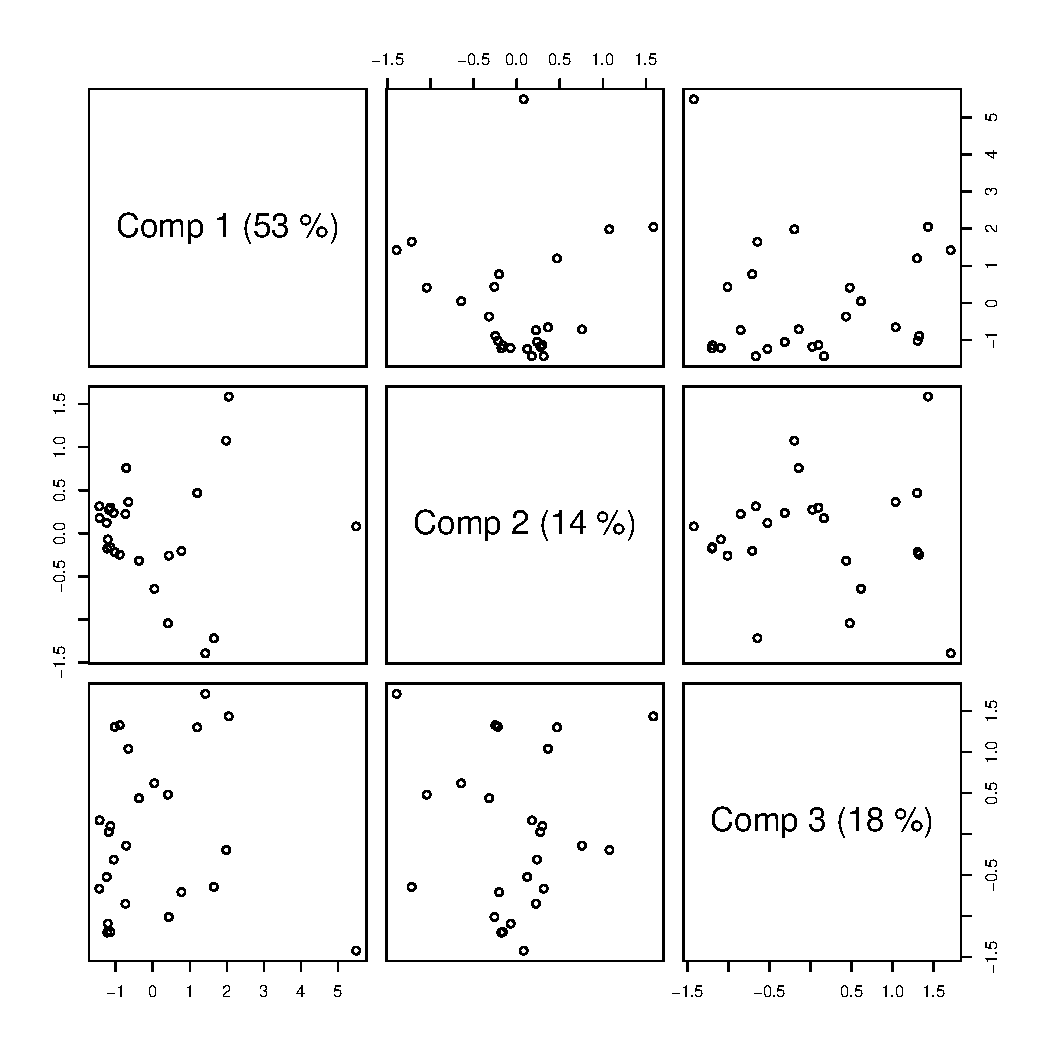
\includegraphics[width=\maxwidth]{figure/unnamed-chunk-19-1} 

\end{knitrout}

\item

\begin{knitrout}
\definecolor{shadecolor}{rgb}{0.969, 0.969, 0.969}\color{fgcolor}\begin{kframe}
\begin{alltt}
  \hlstd{Radj} \hlkwb{=} \hlkwd{c}\hlstd{(}\hlnum{0}\hlstd{,} \hlnum{95.1} \hlstd{,}   \hlnum{95.21}  \hlstd{,}  \hlnum{96.61}  \hlstd{,}  \hlnum{98.05} \hlstd{,} \hlnum{98.05}\hlstd{)}\hlopt{/}\hlnum{100}
  \hlstd{n} \hlkwb{=} \hlnum{25}
  \hlstd{ans} \hlkwb{=} \hlkwd{integer}\hlstd{(}\hlnum{5}\hlstd{)}
  \hlkwa{for} \hlstd{(i} \hlkwa{in} \hlnum{2}\hlopt{:}\hlnum{6}\hlstd{)}
  \hlstd{\{}
    \hlstd{ans[i}\hlopt{-}\hlnum{1}\hlstd{]} \hlkwb{=} \hlstd{(n}\hlopt{-}\hlstd{i}\hlopt{-}\hlnum{2}\hlstd{)}\hlopt{*}\hlstd{(Radj[i]}\hlopt{-}\hlstd{Radj[i}\hlopt{-}\hlnum{1}\hlstd{])}\hlopt{/}\hlstd{(}\hlnum{1}\hlopt{-}\hlstd{Radj[i])}
  \hlstd{\}}
\end{alltt}
\end{kframe}
\end{knitrout}

\item

\end{enumerate}

\section{Problem 6}

\section{Problem 7}

\section{Problem 8}




\end{document}
